%!TEX encoding = UTF-8 Unicode
%!TEX program = xelatex

\documentclass[bachelor]{ustcthesis}
% bachelor|master|doctor
\usepackage{ustcextra}
\graphicspath{{figures/}}
\bibliographystyle{ustcauthoryear}
% \bibliographystyle{ustcnumerical}


\newcommand{\docname}{软件工程作业}
\renewpagestyle{front}[\zihao{-5}]{
    \sethead{}{\docname 聊天软件需求规格说明书}{}
    \setfoot{}{\thepage}{}
    \headrule
}
\renewpagestyle{main}[\zihao{-5}]{
    \sethead{}{\docname 需求规格说明书}{}
    \setfoot{}{\thepage}{}
    \headrule
}
\newcommand{\HRule}{\rule{\linewidth}{0.5mm}}

\begin{document}



\begin{titlepage}
\begin{center}
~\\[5cm]
\HRule \\[0.4cm]
{\huge \bfseries \docname\\需求规格说明书}\\[0.4cm]
\HRule \\[1.5cm]

\begin{tabular}{ccc}
  & 人员 & 日期 \\
<<<<<<< Updated upstream
拟制 & 郑非 \ 钱劲翔 \ 邢宇 & 2018-04-30 \\
=======
拟制 & 郑非\ 钱劲翔\ 邢宇 & 2018/04/30 \\
>>>>>>> Stashed changes
\end{tabular}

\end{center}
\end{titlepage}



\frontmatter
\begin{abstract}
本文是软件工程需求规格说明书模板,修改自于中国科学技术大学本硕博毕业论文 \LaTeX{} 模板示例文件,该模板由
zepinglee和seisman创建,遵循中国科学技术大学的论文写作规范,适用于撰写学士、硕士和博士学位论文。

本文档最后一章演示如何使用 \LaTeX{} 的一些基本命令以及本模板提供的一些特殊功能,
模板的选项及详细用法请参考模板说明文档 ustcthesis.pdf。请在提交之前把最后一掌实例注释掉。

\keywords{软件工程\zhspace{} 中国科学技术大学\zhspace{} 学位论文\zhspace{} \LaTeX{}~通用模板\zhspace{} 学士\zhspace{}
硕士\zhspace{} 博士\zhspace{} 示例文档\zhspace{} 模板说明文档}

\begin{table}[htbp]
\centering
\caption{缩略词清单} \label{tab:simpletable}
\begin{tabular}{|c|c|c|}
    \hline
    缩略语 & 英文全名 & 中文解释 \\
    \hline
    c & d & e\\
    \hline
\end{tabular}
\end{table}

\end{abstract}

\tableofcontents
\listoffigures
\listoftables
% \listofalgorithms  % 算法索引,如不需要,可直接注释掉本行
% \begin{notation}

%\centering
%XX 软件需求规格说明书

%关键词:能够体现文档描述内容主要方面的词汇。
 
%摘要:


\centering
\begin{tabular}{rl}
$\ln x$ & natural logarithm $\log_ex$ \\
$\log x$ & common logarithm $\log_{10}x$ \\
$x\ \mathrm{mod}\ y$ & remainder \\
\end{tabular}

\end{notation}


\mainmatter
\chapter{简介}
\section{目的}


本需求文档主要为软件开发者所制作,意在指明即时通讯软件系统(以下简称通讯系统)的开发需求和具体实现方向。

本文档还可作为软件开发过程中的备案,为后续需求的提出给出参考。此外,非软件开发者可以将这个文件视为我们的即时通讯系统的开发纲要。

\section{范围}


本文档主要包括
\begin{enumerate}
	\item 通讯系统的总体概述
	
	\item 通讯系统的具体需求
	
	\item 通讯系统的设计约束
	
	\item 通讯系统的软件质量特性
	
	\item 通讯系统的其它要求
	
	\item 通讯系统的依赖关系
	
	\item 通讯系统的需求分级
	
	\item 其它待定问题 
\end{enumerate}

对应的,本文档除去上述内容之外,不会包含设计理念、实现方法、开发过程等细节上的问题。

\chapter{任务概述}
本系统的目标是实现一个xxx系统,包括客户端、服务器端两个部分。

客户端面向xxx用户,为用户提供xx和xx服务。

\section{目标}
实现xxx系统,实现需求规格说明书中所描述的xx功能、xxx功能和xxx功能,并且保证系统的健壮性和数据安全。

\section{开发与运行环境}

\subsection{开发环境的配置}
\begin{table}[htbp]
\centering
\caption{开发环境的配置} \label{tab:development-environment}
\begin{tabular}{|c|c|c|}
    \hline
    类别 & 标准配置 & 最低配置 \\
    \hline
    计算机硬件 & \tabincell{c}{基于x86结构的CPU\\ 主频>=2.4GHz\\ 内存>=8G\\ 硬盘>=200G} & \tabincell{c}{基于x86结构的CPU\\ 主频>=1.6GHz\\ 内存>=512M\\ 硬盘>=2G} \\
    \hline
    计算机软件 & \tabincell{c}{Linux (kernel version>=4.10)\\ GNU gcc (version>=6.3.1)} & \tabincell{c}{Linux (kernel version>=3.10)\\ GNU gcc (version>=5.4)} \\
    \hline
    网络通信 & \tabincell{c}{至少要有一块可用网卡\\ 能运行IP协议栈即可} & \tabincell{c}{至少要有一块可用网卡\\ 能运行IP协议栈即可} \\
    \hline
    其他 & 采用MySQL数据库 & 采用MySQL数据库 \\
    \hline
\end{tabular}
% \note{这里是表的注释}
\end{table}

\section{需求概述}
功能需求包括:


\section{条件与限制}
本节至少要与需求说明文档中相关章节相一致。

\chapter{具体需求}
\iffalse
<The following sections must be repeated for each requirement. >

在每一条需求描述中重复下列部分
\fi
\section{功能需求}
\iffalse
This section describes how the input of the software is translated to the output. It describes the essential action the software must perform.

For each kind of function, or each independent function in some cases, the requirements of input, process and output must be described, which are usually organized with the following four subsections:

本子章节应描述软件产品的输入怎样被转换成输出。它描述了软件必须执行的基本动作。

对每一类功能或有时对每一个单独的功能,必须描述输入、处理、输出方面的需求。这些通常以下面四个子段落来组织:
\fi
\subsection{Android客户端功能需求}
\subsubsection{简介}
随着Android平台日益普及,Android客户端是该即时通讯产品的主要客户端,拥有该产品的所有完整功能。
\begin{itemize}
\item 通讯模式
  \begin{itemize}  	
  	\item 用户一对一通讯
  	\item 群聊
  	\item 随机匹配聊天
  \end{itemize}
\item 通讯方式
  \begin{itemize}
  	\item 文字即时通讯
  	\item 图片、视频、音频、链接、文件等多媒体消息的发送
  	\item 语音、视频即时通讯
  	\item 加密文字即时通讯
  \end{itemize}
\item 用户控制
  \begin{itemize}
  	\item 注册/注销账号
    \item 找回或修改密码
  	\item 添加/删除联系人
  	\item 加入/退出/创建群聊
    \item 选择登录状态 在线/隐身/忙碌 
  \end{itemize}
\end{itemize}
  \begin{figure}[!h]
	\includegraphics[width=8cm]{Page0}
	\includegraphics[width=8cm]{Page1}
	\includegraphics[width=8cm]{Page2_0}
	\includegraphics[width=8cm]{Page2_1}
	四张图分别对应 启动页面、登录页面、群聊页面和会画页面
	\label{fig:noted-figure}
   \end{figure}
\subsubsection{启动}
  点击本APP的图标之后,启动项目,首页会显示图片和两个按钮,分别是连接和退出。
\subsubsection{连接}
  点击连接图标之后,如果连接成功,则登录到主界面。
\subsubsection{登录和注册}
  在主界面输入用户名、密码即可登录,如果没有注册,则可以点击“注册”按钮进行注册。一旦注册,则账号和密码被存储到服务器数据库中。
\subsubsection{创建会话}
  登陆之后就可以创建会话、群聊。在上方菜单栏可以选择群聊或会话。通过点击用户列表中的用户就可以发起会话。
\subsubsection{会话界面}
  用户可以在输入框里输入文字并且发送。\\
  用户通过点击最下面的一栏菜单的相应按钮,用户可以发送语音、图片、文件等信息。也可以发起语音通话和视频聊天。
  \begin{figure}[!h]
  	\centering
	\includegraphics[width=9cm]{Page3}
	\note{聊天界面}
	\label{fig:noted-figure}
  \end{figure}

\section{性能需求}
\iffalse
<If there are performance requirements, state them here and explain their rationale, to help the developers understand the intent and make suitable design choices. Specifies the timing relationships for real time systems. Such requirements should be made as specific as possible. >

如果有性能方面的需求,在这里列出并解释他们的原理。以帮助开发者理解意图以做出正确的设计选择。在实时系统中的时序关系。保证需求尽可能的详细而精确。

\subsection{性能需求1}
Describes the statically and dynamically quantized requirements on the software (or the interaction between user and the software)
Static quantized requirement could include:
A. Maximum number of terminal supported.
B. Maximum number of users that can use the software at the same time.
C. Maximum number of files and records to be processed
D. Maximum size of  tables and files
Dynamically quantized requirements could include:
A. Specific duration of normal value and peak value of workload (e.g., one hour)
B. Number of event and task and data volume to be processed
All these requirements should be described by measurable term, for example, saying "95% of the events should be processed in 1 second", instead of saying "the operator need not wait for the business to complete."
Note: The quantized constraint of a detailed requirement should be described in the subsection of the detailed requirement.
本子章节应从整体上描述静态和动态的量化的对软件(或人与软件交互)的需求。

静态的量化需求可能包括:

A. 支持的终端数目。

B. 支持的同时使用的用户数目。

C.处理的文件和记录的数目。

D.表和文件的大小。

动态的量化需求可能包括:

A. 在正常和峰值工作量条件下特定时间段(如一小时)

B. 处理的事务和任务的数目以及数据量。

所有的这些需求应以可测量的术语进行描述,例如所有的操作应在1秒内被处理完成,而不是描述成操作员不必等待操作的完成。

注意: 用于一个具体功能的量化限制通常在该功能的处理子章节中描述。
\fi
\subsection{服务器端性能需求}
\begin{itemize}
	\item 稳定性要求:服务器有效工作时间在99.5\%以上,每次维护时间<24小时。
	\item 业务处理性能要求:能够满足>300个人同时在线,并且满足>50对人能够同时进行较为流畅的视频聊天。据此估算,需要服务器带宽 > 300Mbps。
	\item 数据库性能要求:数据库每秒钟能够进行>400次查询、修改、删除操作,对于每次操作,从收到客户端请求到响应的时间应该小于20ms。
\end{itemize}
\subsection{Android客户端性能需求}
\begin{itemize}
	\item UI界面能够及时响应用户的触摸、点击等事件
	\item 在网络良好的情况下,用户接收、发送消息的延迟<100ms。
	\item 对内存的占用<100MB,不考虑用户文件的情况下,对存储空间的占用<100MB.
	\item 在客户端连续工作的情况下,1小时的耗电量不超过手机基础耗电量的200\%。注:基础耗电量指的是不打开任何外部应用,屏幕开启的情况下手机的耗电量。
	\item 在客户端连续工作的情况下,手机温度相比于未打开客户端的情况没有明显提升。
\end{itemize}
\section{外部接口需求}
\subsection{用户接口}
\iffalse
<The interface of the system with the User and vice versa should be explained in detail. >

详细描述系统与用户之间的接口

This section should include:
A. Features that must be supported by the software for eachman-machine interface. For example, if the user operates from a display terminal, then the following should be included:
		Screen format required
		Page layout and content of report and menu
		Timing sequence for input and output
		Usage of some functional key combinations
B. Every aspect about the use of the system's user interface. It could be a list that shows the user what should do and what should not do.  For example, an option of overlong or overshort message. . And same as other requirements, these requirements should be easily verified. For example, saying "A level 4 typist can finish function X in Z minutes after a one-hour training." instead of "A typist can finish function X"	

这应描述下述内容:

A. 对每种人机界面,软件所必须支持的特性。例如,如果系统用户通过一个显示终端进行操作,那么应包含下述内容:
要求的屏幕格式
页面规划及报告或菜单的内容
输入和输出的相关时序
一些组合功能键的用法

B. 与系统用户接口使用相关的所有方面。这可能只是一个简单的关于系统怎样展示给用户而该做什么和不该做什么的列表。例如提供关于长或短错误消息选项。和所有其它需求一样,这些需求也应能被检验,例如,四级打字员经一小时的培训后能在Z分钟内完成功能X,而不是一个打字员能完成功能X。
\fi
在功能需求里已经详细叙述用户接口。
\begin{itemize}
	\item 需要屏幕分辨率$\ge$800$\times$600, 支持16位以上颜色显示
\end{itemize}
\subsection{软件接口}
\iffalse
<The interface with other system/modules/projects should be explained in detail. >

详细描述与其他系统 /模块 /项目之间的接口

Describes how to use the other (required) software products. (such as data management system, operation system, or algorithm tools package), and the interfaces to other application systems (such as interfaces between the protocol process system and the database management system )
For each required software product, following information should be provided:
A. Name
B. Mnemonic symbol
C. Version number
D. Source
For each interface, this section should:
A. Discuss the objective of the required software.
B. Define the interfaces by content and format of message/function. If the interfaces have been clearly described in other documents, it is not necessary to describe in detail here. But the reference of those documents should be given.

在此应描述如何使用其它(必需的)软件产品(例如,数据管理系统,操作系统,或算法工具包),以及与其它应用系统的接口(例如,协议处理系统和数据库管理系统之间的接口)。

对每个必需的软件产品,应提供下列信息:
A.	名字
B.	助记符
C.	版本号
D.	来源

对每个接口,本部分应:

A .	讨论与本软件产品相关的接口软件的目的。

B.	按消息/函数内容和格式定义接口。如果接口已在其它文档中很清楚地描述,就没有必要在这儿进行详细描述,但需说明应参考的文档。
\fi
\begin{itemize}
\item 客户端
	\begin{itemize}
	\item Windows操作系统(XP以上版本,包含.Net4.0组件)
	\item Android操作系统(5.0.1以上版本)
	\end{itemize}
\item 服务器端
	\begin{itemize}
	\item Ubuntu Server 16.04 操作系统
	\item Mysql数据库
	\item Apache2.0服务器
	\end{itemize}
\end{itemize}




\subsection{硬件接口}
\iffalse
<The interface with other hardware components should be explained in detail. >

详细描述与硬件的接口

Describes the logical features of the interface between the software and hardware components, including the equipment supported and how the equipment and protocol is supported.

Defines the interfaces according to the content and format of the software/hardware protocol. If the interfaces have been clearly described in other documents, it is not necessary to describe in detail here. But the reference of those documents should be given.

在此描述软件产品和系统硬件组件之间接口的逻辑特征,也包括支持哪些设备、怎样支持这些设备和协议等。

按软/硬件协议内容和格式定义接口。如果接口已在其它文档中很清楚地描述,就没有必要在这儿进行详细描述,但需说明应参考的文档。
\fi
\begin{itemize}
	\item 客户端
	\begin{itemize}
		\item 屏幕分辨率$\ge$800$\times$600的手机
		\item 支持麦克风、扬声器或耳机接口
		\item 具有前置摄像头
	\end{itemize}
	\item 服务器端
	\begin{itemize}
		\item 云服务器,含有$\ge$500GB的云硬盘
		\item 具有公共网络接入点
	\end{itemize}
\end{itemize}
\subsection{通讯接口}
\iffalse
<This should specify the various interfaces to communications such as local network protocols, etc.>

详细描述通讯接口,如本地网络协议等。

Defines the interfaces according to the content and format of the message/function. If the interfaces have been clearly described in other documents, it is not necessary to describe in detail here. But the reference of those documents should be given.

按消息/函数内容和格式定义接口。如果接口已在其它文档中很清楚地描述,就没有必要在这儿进行详细描述,但需说明应参考的文档。
\fi
所有信息通过TCP协议发送,要求客户端和服务器支持TCP传输。
\begin{itemize}
	\item 客户端-服务器事件交互信息,采取如下Json字符串格式
    \begin{lstlisting}[language=C++]
   	{
   		"Sender":"sender_id",
   		"SendTime":"send_time",
   		"EventCode":"event_code",
   		"EventParas":
   		{
   			"para1":"para_1",
   			"para2":"para_2"
   		}
   	}
    \end{lstlisting}
    \item 客户端-客户端消息类信息,在头部加上消息发送方、接收方等信息。
    \begin{lstlisting}[language=C++]
    sender_id(32bits)
    receiver_id(32bits)
    datetime(32bits)
    length(32bits)
    payload
    \end{lstlisting}
\end{itemize}

\chapter{总体设计约束}


对于开发人员可能的限制有:来自国内或者国际上的标准
硬件的条件
开发技术的约束
具体实现上的约束
 
\section{标准符合性}


本章所遵循的设计原则均来源于IEEE对通讯系统和数据库的标准,所假定的硬件均为当下一般民众的平均水平,并且所有的行为是在相关法律法规的允许之下执行的。


\section{硬件约束}

\begin{enumerate}
	\item Android平台:软件本身大小<100MB;本地聊天记录文件不大于1G,并且有着自动清除过时的聊天记录功能;文本通信延迟<100ms;内存占用<100MB;流量消耗不超过通信本身数据量的1.1倍;电量消耗不超过机体待机时的两倍
	\item Windoes平台:约束较少,主要考虑的磁盘和内存约束与Android一致。
\end{enumerate}

\section{技术限制}

\begin{enumerate}
	\item 考虑到服务器网络带宽问题,视频聊天的清晰度最高维持在360P;
	\item 
	由于技术上的限制,除去文本类的通信记录都不会被保存;
	\item
	用户无法在不同的客户端上共享聊天记录;
	\item
	用户无法在周日凌晨2:00至4:00使用通讯软件的聊天功能因为这个时候应该是维护服务器的时候;
	\item 
	由于服务器磁盘大小的限制,用户传输文件的大小有着<8MB的限制
	
\end{enumerate}

\section{实现功能约束}

\chapter{软件质量特性}
<<<<<<< Updated upstream

=======
/iffalse
<Specify any additional quality characteristics for the project that will be important to either the customers or the developers. Some to consider are: adaptability, availability, correctness, flexibility, interoperability, maintainability, portability, reliability, reusability, robustness, testability, and usability. Write these to be specific, quantitative, and verifiable when possible. At the least, clarify the relative preferences for various attributes, such as ease of use over ease of learning.
>>>>>>> Stashed changes

详细说明项目任何其他的质量特性。该特性对客户和开发者都非常重要。考虑的方面包括:适应性,可用性,正确性,灵活性,交互工作能力,可维护性,可移植性,可靠性,可重用性,鲁棒性,可测试性和可用性等。定量的详细描述这些特性,尽可能的可验证。对不同属性之间的重要性加以阐述,如:易用性比易学性更重要。


<<<<<<< Updated upstream

\section{适应性}
考虑到Android平台本身的共通性,通讯系统能正常的运行在绝大部分的Android5.0.1及以上版本的机器上。至于windows平台,则支持xp及以上的操作系统,需要包含微软提供的.Net4.0的组件即可。


\section{交互工作能力}
通讯系统有着完整的用户友好的UI,易于上手。

\section{灵活性}
通讯系统既可以和好友一对一交流,又可以在群组多对多交流,还可以随机配对,和大厅里的任何一个用户交流。

\section{可维护性}
由于用户端和服务器端的分离,用户端的升级只需要通过软件提供商更新安装包就可以了。而后台服务器端则是至少24小时备份一次数据库,至少每周进行一次人工维护。并且所有维护均会留下维护记录,所有的错误信息也会留下log,可维护性得以保障。

\section{可移植性}
通讯系统由Java开发,我们不仅准备了Android和Windows的两种版本,也使得打包封装和移植到别的系统简单。

\section{可测试性}
通讯系统提供了专门用于测试的接口,并且还会提供开发中的各种中间版本作为升级记录。

\section{安全可靠性}
通讯系统在http,tcp等网络传输协议之外,发送的报文还会进行一层RSA加密,大大增强信息的安全性。此外对于绑定邮箱的用户还会有额外的异常登录验证,确保用户账户的安全性。并且开发人员绝不会收集用户的信息和聊天记录,通讯系统是一个绝对的绿色安全可靠的软件。

=======
每一个属性单独使用一个小节描述,可根据需要进行增减,如增加可维护性小节等。
/if
>>>>>>> Stashed changes

\chapter{其他需求}
\iffalse
<Any other requirement specified by the customer need to be listed below with appropriate section. This may include Database, Coding requirements, Error handling, Testing requirements etc., Few sample requirements are listed below. Please note, you may remove or add if something is not applicable. >

使用适当的章节,详细说明任何其他客户需求,包括数据库,编码需求,错误处理,测试需求等。下面仅列出了少量样例,你可以删除和增加项目。
\fi
\section{数据库}
考虑到通信数据的传输问题,通讯系统需要数据库的支持。又通讯系统决定考虑不云端对用户聊天信息的存储,仅存储用户的基本信息,故对数据库的需求并不是很大,相信只需要一台云端服务器就可以胜任。同时还要考虑语音信息乃至视频信息的传输,故对云端服务器带宽要求较高。
\section{操作}
%<This could specify the normal and special operations required by the user. >
用户输入支持键盘和手写。键盘支持第三方键盘app。图片消息传输需要用户提供访问图片库的权限。试试视频和语音需要用户提供摄像头和麦克风的权限。
\section{本地化}
%<Any requirement on multi language operation could be described here. >
目前界面语言支持中英文。用户接口大多采用符号,故对其他语言的使用影响不大。消息的发送支持任何符号语言。
\section{编码}
用户名和密码验证采取base64编码。用户消息采用UTF-8编码后加密。音频编码采取G.722标准。视频采取H.264编码标准

\chapter{依赖关系}



\section{功能需求}
\subsection{Android客户端功能要求}
\section{内部依赖}
客户提出的各种要求,同时外部需要满足Android操作系统的支持。

\section{性能需求}

\subsection{服务器端性能要求}
\section{内部依赖}
对服务器性能的分析和消耗的优化,外部依赖稳定的云服务器(主要是存储和转发)。
\subsection{Android端性能要求}
内部依赖对Android操作系统性能的分析和消耗的优化,外部依赖可靠的稳定的Android系统和搭载设备。

\section{接口需求}

\subsection{用户接口}
用户接口只依赖用户提出的要求。
\subsection{软件接口}
\section{内部依赖}
用户接口要求,性能要求和功能要求

\section{外部依赖}
Android操作系统和Windows系统给出的接口规范。
\subsection{硬件接口}
\section{内部依赖}
软件接口

\section{外部依赖}
搭载了Android操作系统的智能手机或者是Windows操作系统的电脑给出的接口规范。
\subsection{通信接口}
\section{内部依赖}
软件接口

\section{外部依赖}
各类网络协议给出的通信规范。
\chapter{需求分级}
\begin{table}[htbp]
\centering
\caption{需求分级表} \label{tab:classification}
\begin{tabular}{|c|c|c|}
    \hline
    需求ID & 需求名称 & 需求分级 \\
    \hline
    R.IM.LOGIN.001  & 用户登录认证 & Mandatory \\
    \hline
    R.IM.LOGIN.002 & 用户登出 & Mandatory \\
    \hline
    R.IM.FUNC.001 & 用户一对一通信 & Mandatory \\
    \hline
    R.IM.FUNC.002 & 用户群组通信 & Mandatory \\
    \hline
    R.IM.EX.001 & 通信安全加密 & Important \\
    \hline
    R.IM.FUNC.003 & 语言聊天 & Important \\
    \hline
    R.IM.FUNC.004 & 视频聊天 & Important \\
    \hline
    R.IM.LOGIN.003 & 记住用户名以及自动登录 & Nice to have \\
    \hline
    R.IM.FUNC.005 & 聊天记录自动同步 & Nice to have \\
    \hline

\end{tabular}
\end{table}


重要性分类如下:
\begin{itemize}
\item 必须的		绝对基本的特性;如果不包含,产品就会被取消。
\item 重要的		不是基本的特性,但这些特性会影响产品的生存能力。
\item 最好有的		期望的特性;但省略一个或多个这样的特性不会影响产品的生存能力
\end{itemize}

\chapter{待确定问题}
\begin{table}[htbp]
\centering
\caption{待确定问题表} \label{tab:tbd_problems}
\begin{tabular}{|c|c|c|c|c|c|c}
    \hline
    需求ID & 问题描述 & 影响(H/M/L) & 风险 & 责任人 & 解决日期  \\
    \hline
    1 & 消息传输加密通道和算法 & H &用户隐私泄露 & 邢宇 & 05/01\\
    \hline
    2 & IOS平台支持 & L & 无风险 & 邢宇 & 05/03\\
    \hline
    3 & 语音消息去环境噪声 & M & 无效消息  & 郑非 & 05/07\\
    \hline
\end{tabular}
\end{table} 
\input{chapters/latex_examples}
\bibliography{bib/tex}









\appendix
\chapter{可行性分析结果}
\iffalse
Describe the feasibility analysis results on allocated requirements.

描述对分配需求的可行性分析结果。
\fi
\begin{table}[htbp]
\centering
\caption{可行性分析} \label{tab:tbd_problems}
\begin{tabular}{|c|c|c|c|}
    \hline
    功能 & 技术可行性 & 经济可行性 & 操作可行性  \\
    \hline
    高质量视频通信 & 需要对延迟、码率、协议的研究 & 对服务器带宽和通信质量的要求 & 获取用户权限\\
    \hline
    聊天消息漫游 & 多设备支持,设备识别,记录同步 & 数据库支持 & 无需用户操作\\
    \hline
    通信加密 & 加密算法的研究 & 经济可行 & 无需用户操作  \\
    \hline
\end{tabular}
\end{table} 

\chapter{需求建模 }
\section{数据流图}
\subsection{顶层数据流图}
\iffalse
<Draw the Top-level DFD here>

在这里画出顶层数据流图
\fi
  \begin{figure}[!h]
  	\centering
	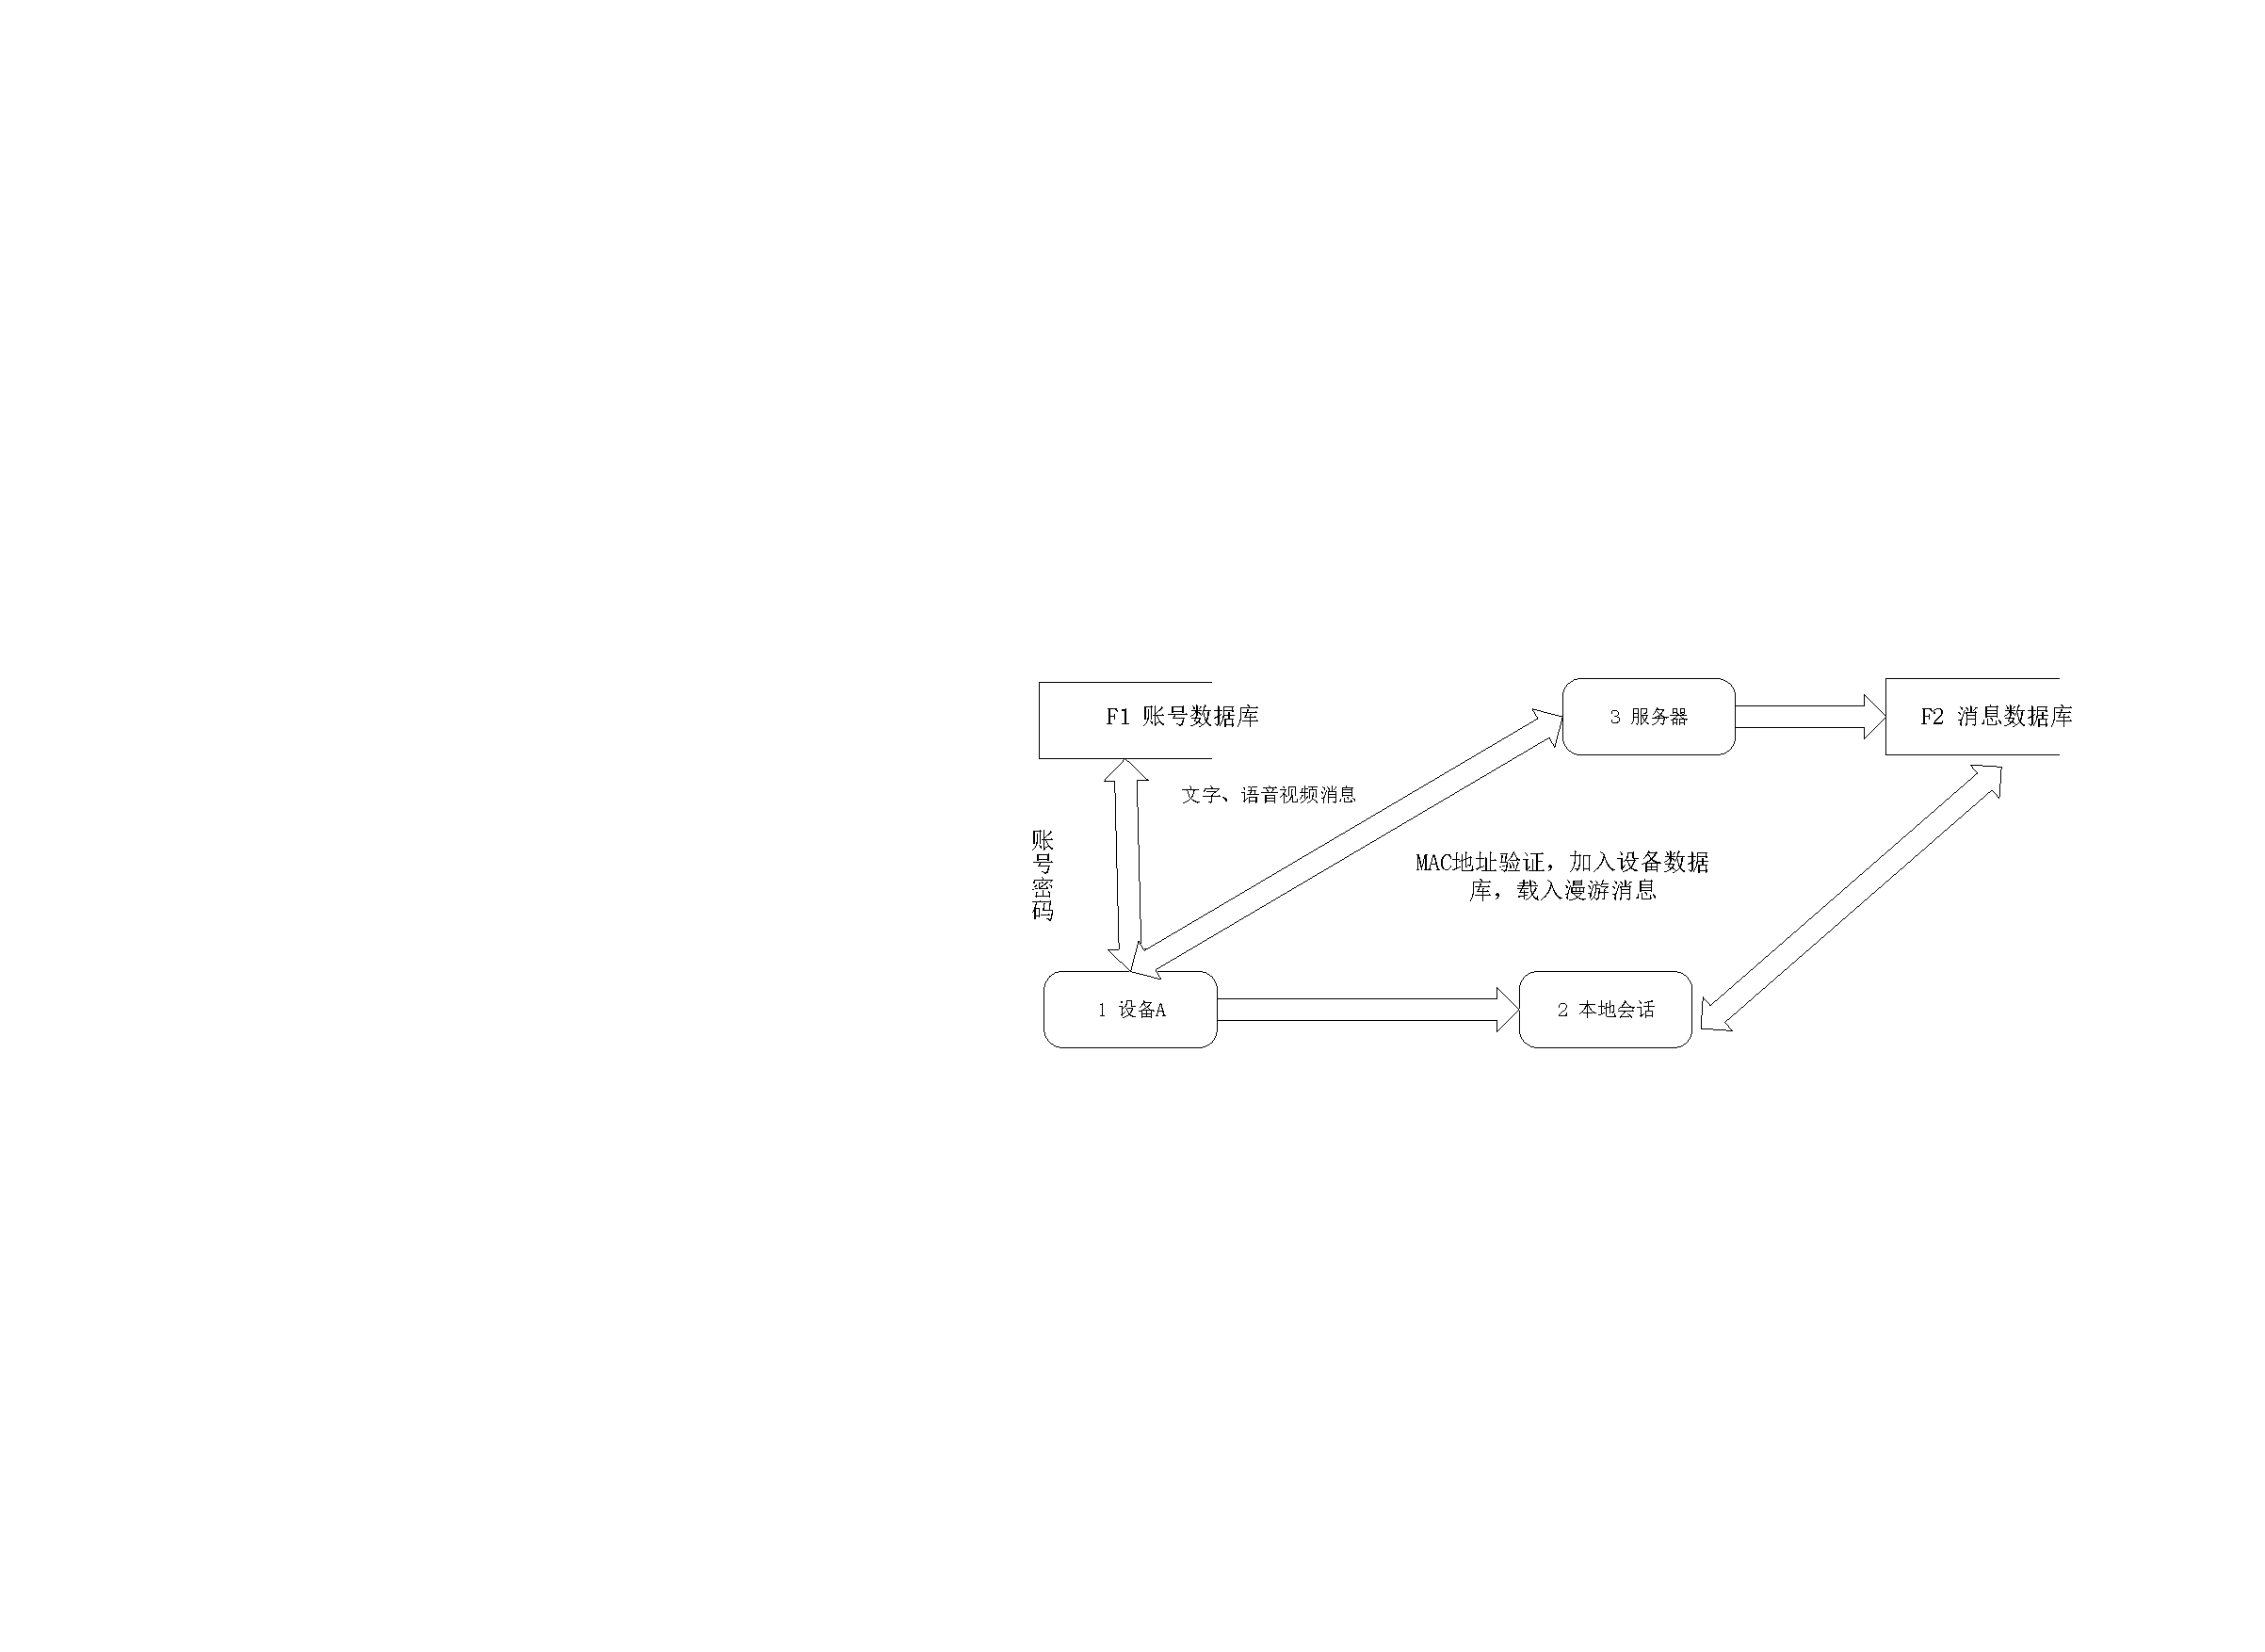
\includegraphics[width=11cm]{DFD}
	\note{顶层数据流图}
	\label{fig:noted-figure}
  \end{figure}
\subsection{层数据流图}
\iffalse
<Draw the Level-0 DFD here>

在这里画出0层数据流图
\fi
  \begin{figure}[!h]
  	\centering
	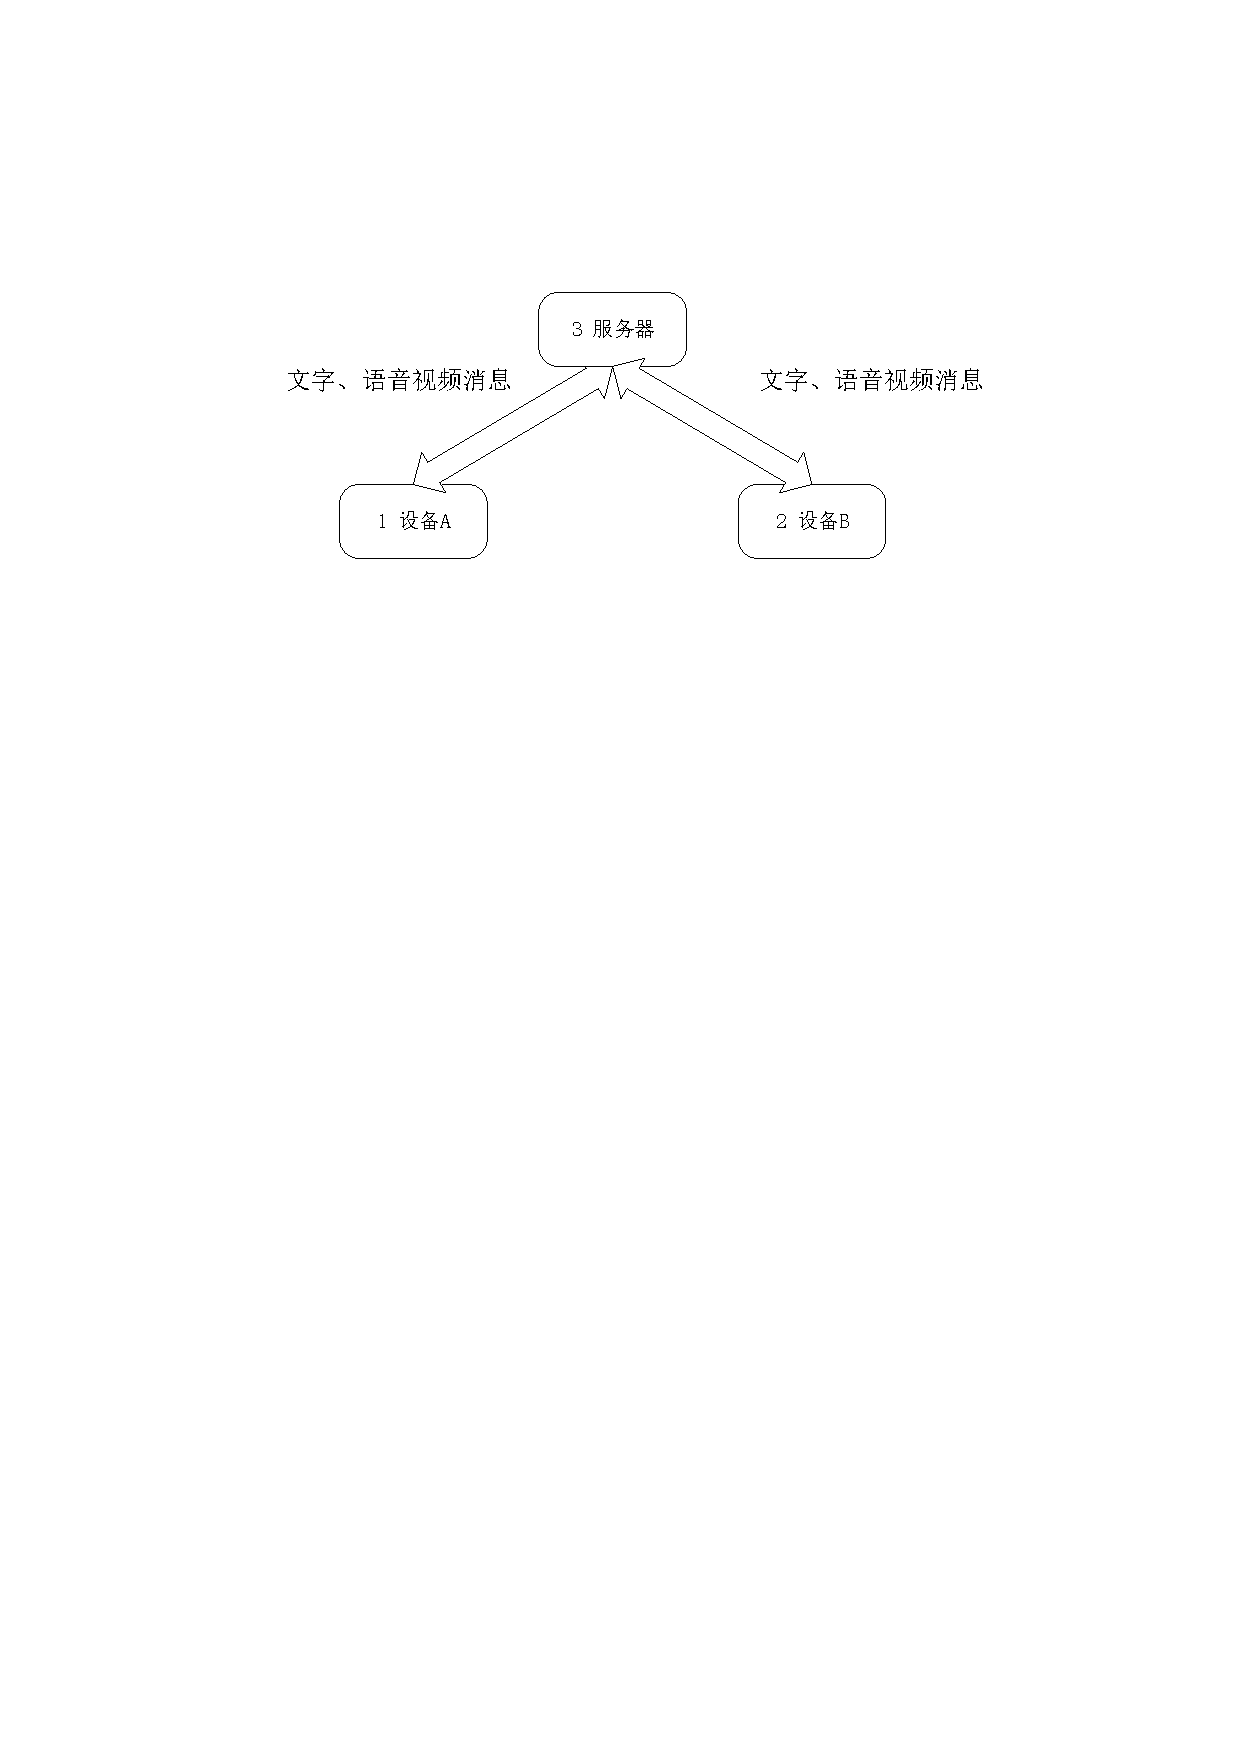
\includegraphics[width=11cm]{levelDFD}
	\note{层数据流图}
	\label{fig:noted-figure}
  \end{figure}

\section{数据字典}
\subsection{数据流说明}
\subsubsection{数据流1名称}
\iffalse
<Title of  the data flow should accord with the one in data flow diagram, and the Data description notions should be used.  >

与数据流图中的名称一致,采用数据描述符号说明数据流的内容
\fi
\subsubsection{数据流2名称}
\iffalse
<Title of  the data flow should accord with the one in data flow diagram, and the Data description notions should be used   >

与数据流图中的名称一致,采用数据描述符号说明数据流的内容
\fi
\subsection{数据存储说明}
\subsubsection{数据存储1名称}
\iffalse
<Title of  the data flow should accord with the one in data flow diagram, and the Data description notions should be used. The arrangement of the data in data store should also be described.>

与数据流图中的名称一致,采用数据描述符号说明数据流的内容,另外还需描述数据排列方式
\fi
F1为用户账号密码经过加密哈希后的数据库。为关系数据模型。数据排列方式为平铺排列。
\subsubsection{数据存储2名称}
\iffalse
<Title of  the data flow should accord with the one in data flow diagram, and the Data description notions should be used.The arrangement of the data in data store should also be described.>

与数据流图中的名称一致,采用数据描述符号说明数据流的内容,另外还需描述数据排列方式
\fi
F2 为用户会话消息数据库
为对象型数据模型,为每个用户对/用户群之间建立关系,将聊天历史文件加密后存储
\subsection{加工说明}
\subsubsection{加工1名称}
\iffalse
<Use natural language, Decision table/Decision tree and Pseudocode to describe how to process the data flow>

采用自然语言,判断表/判断树,伪码的形式描述对数据流进行处理的过程
\fi
处理过程:
账号密码进行加盐处理,并哈希后与F1中已有值比较。本地验证码验证。\\
设备向服务器发出HTTP报文的连接请求,服务器识别设备的mac地址,并将其加入信任列表\\
服务器想消息数据库发送请求,加载包含改用户的所有会话消息\\
服务器用所有会话消息更新设备\\
设备创建本地会话\\
本地会话间隔固定时间加密上传\\



\end{document}
